\documentclass[12pt]{book}
\usepackage{palatino}
\usepackage{epsfig}

\setlength{\topmargin}{0in}
\setlength{\oddsidemargin}{0.2in}
\setlength{\evensidemargin}{0.2in}
\setlength{\textwidth}{6.4in}
\setlength{\textheight}{9in}
\setlength{\parindent}{0in}
\setlength{\parskip}{0.1in}
\pagestyle{empty}

\begin{document}
  
  \begin{center}
    {\LARGE \bf DUMNEZEIASCA LITURGHIE\\
      \vspace{0.1in}
      \^{I}n Duminici \c{s}i S\u{a}rb\u{a}tori}
  \end{center}

  \vspace{0.5in}
  
  {\bf Preotul:} Binecuv\^{a}ntat\u{a} este \^{i}mp\u{a}r\u{a}\c{t}ia
  Tat\u{a}lui \c{s}i a Fiului \c{s}i a Sf\^{a}ntului Duh, acum \c{s}i
  pururea \c{s}i \^{i}n vecii vecilor.

  {\bf Cantorul:}
  \begin{figure}[h]
    \begin{center}
      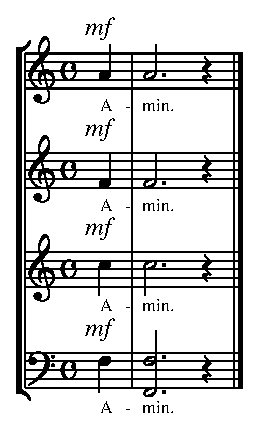
\epsfig{file=amin_1.eps}
    \end{center}
  \end{figure}

  {\bf Preotul:} Cu pace, Domnului s\u{a} ne rug\u{a}m.

  {\bf Cantorul:}
  \begin{figure}[h]
    \begin{center}
      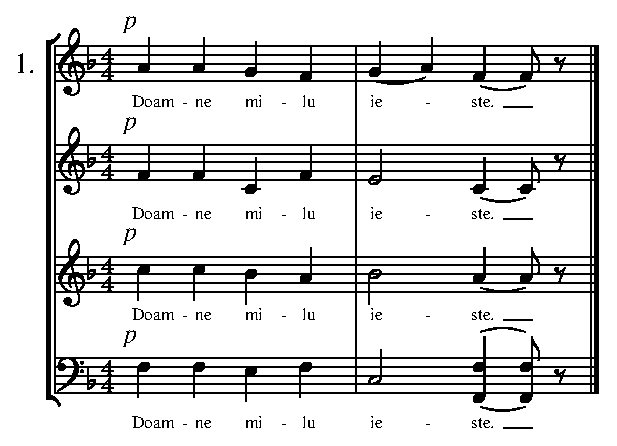
\epsfig{file=dm_1.eps}
    \end{center}
  \end{figure}

\pagebreak
\pagestyle{myheadings} \markright{\hfill \small } \setcounter{page}{1}


\end{document}
